\chapter{System architecture}

\paragraph*{To implement our project we are using the following softwares :} 
\begin{enumerate}
\setlength{\itemsep}{-0.3em}
\item Eclipse : To implement the project
\item Pgsql : To store Unix commands and its description in database
\end{enumerate}

\vspace*{3 ex}

Both the above mentioned software are open source softwares so, the project implementation is free of cost.\\ \\
For Graphical User Interface (GUI), swing components of java are used. GUI for game consists of one 10x10 matrix and two text area, one to display hint and other one to dispaly solution for the puzzle.\\ \\
The "postgres" SQL is used to store words i.e unix commands and its description that are used to generate crossword puzzle. Words are used to generate crossword puzzle and descriptions are used to generate hint for the game.\\ \\


\section{Design}
\vspace*{3 ex}
In the process of crossword puzzle generation, first of all the words are extracted from database and stored in string array; among the extracted words, eight words and its hint are are randomly selected in sequence (order in which they are stored in database) and stored in string arrays. These words are than feeded to the crossword puzzle generator algorithm which result in 10x10 matrix puzzle generation. The generated game is finally displayed in GUI 10x10 matrix and hints are displayed in text frame. After submittimg the solution by user the correct solution will be dispalyed.\vspace*{7 ex}

%\vspace*{3 ex}
\textbf{PROJECT LAYOUT :}


Here is the layout of CROSSWORD PUZZLE generator and schema of database used in this project :\\
\begin{figure}[!ht]
\centering
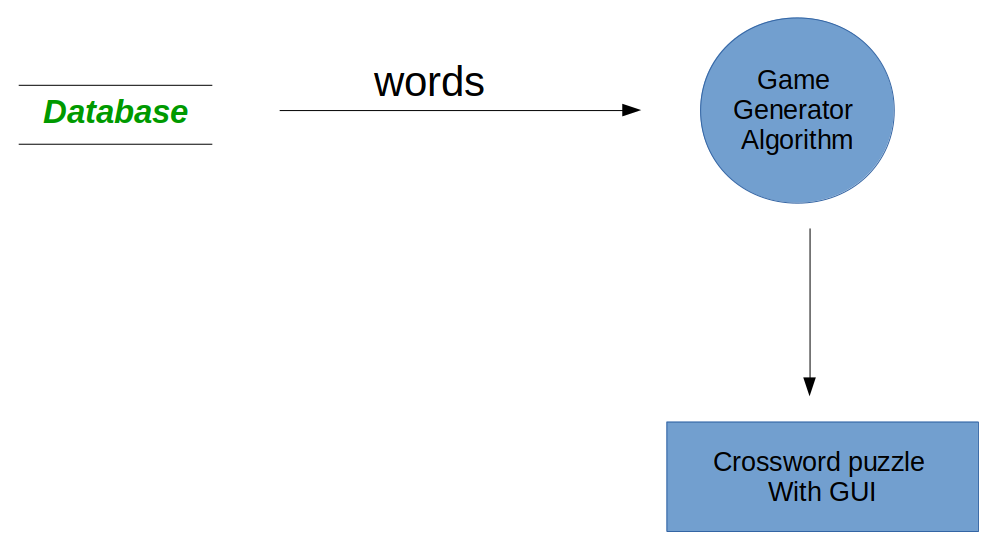
\includegraphics[scale=0.4]{layout.png}
\caption{\label{img} Project Layout}
\end{figure}

%\vspace*{3 ex}

\begin{figure}[!ht]
\centering
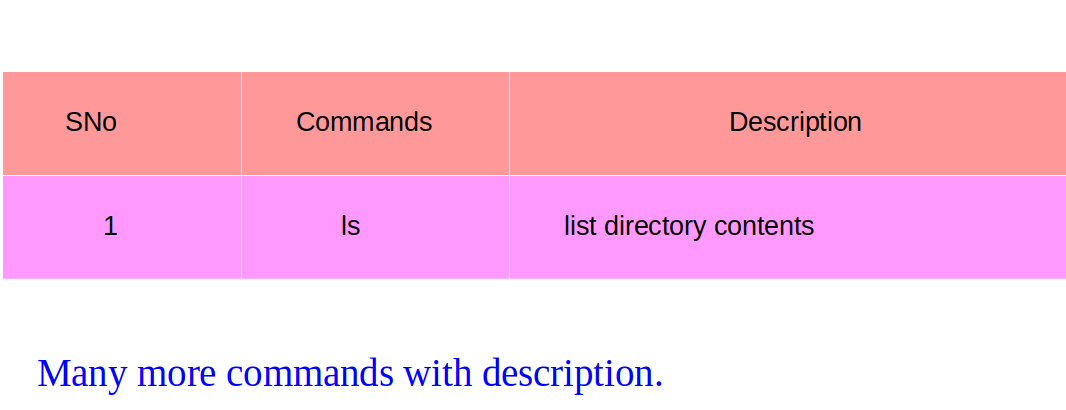
\includegraphics[scale=0.4]{db.png}
\caption{\label{img} DB schema}
\end{figure}



%\begin{figure}[!ht]
%\centering
%\includegraphics[scale=0.9]{car1.png}
%\caption{\label{img5} Entity relation ship diagram}
%\end{figure}

